%!TEX root = IS_0_s1234567_s2345678.tex



\begin{figure}[htbp] 
    \centering
    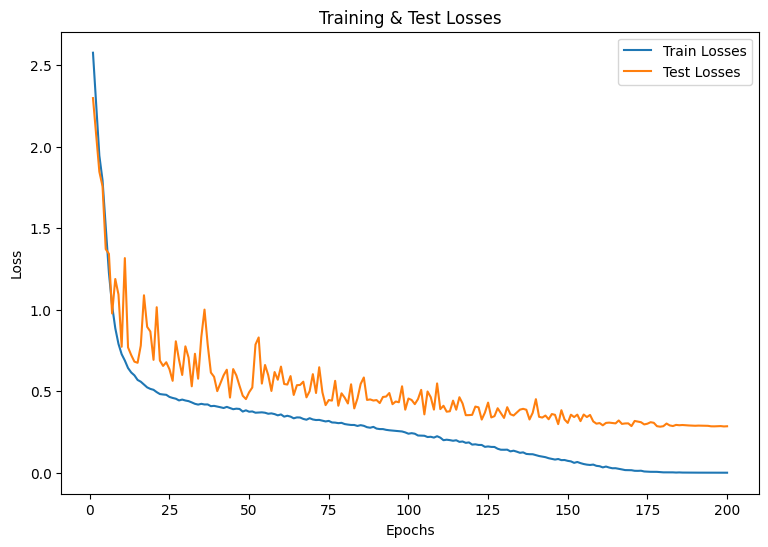
\includegraphics[width=1\textwidth]{images/ex_1_loss} 
    \caption{Plot of the average training loss per epoch compared to the average test loss per epoch.}
\end{figure}

\begin{figure}[htbp] 
   \centering
   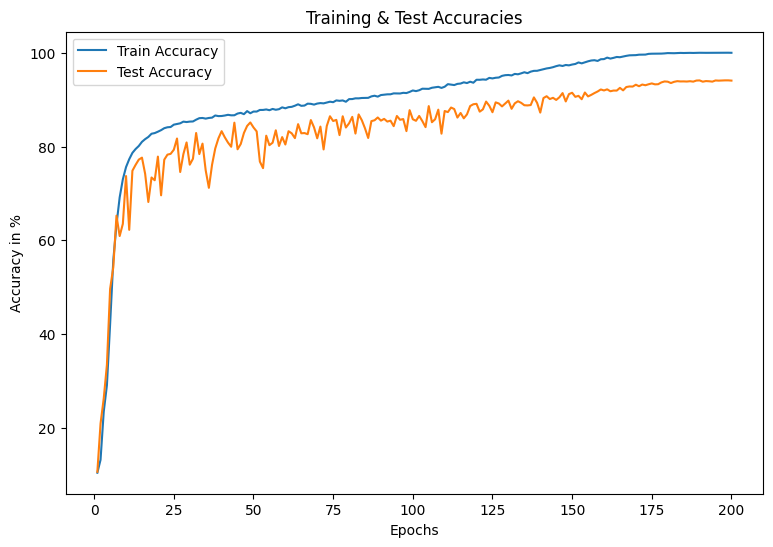
\includegraphics[width=1\textwidth]{images/ex_1_acc} 
   \caption{Plot of the average training accuracy per epoch compared to the average test accuracy per epoch.}
\end{figure}











% Example code from the boilerplate 
%\begin{enumerate}
%	\item 
%		Some equation can be found in \eqref{eq:1:einstein}, \autoref{fig:1:1:someFigure} could show an image.
%
%		\begin{equation}\label{eq:1:einstein}
%			E = mc^2
%		\end{equation}
%		You can add inline code using the shortcut e.g: \t{int a = 7}. If you want to use a code block use:
%		\begin{lstlisting}[caption={Somde code block}, label={lst:1:someCode}]
%			int a = 7;
%		\end{lstlisting}
%		You can then refer to it using \autoref{lst:1:someCode}. To denote the absolute value of a number use $\abs{7}$, use $\norm{\vec{a}}$ for the norm of vector $\vec{a}$. For this course we use the book \textcite{duda2012pattern} by \citeauthor{duda2012pattern}.
%
%		\begin{figure}
%			\centering
%			\missingfigure{Add your figure by changing the file path in includegraphics.}
%			% \includegraphics[width=\textwidth]{./img/_}
%			\caption{Caption here}
%			\label{fig:1:1:someFigure}
%		\end{figure}
%	\item \todo[inline]{rinse and repeat}
%\end{enumerate}
%The code used to complete this assignment, that has not been included above, is presented in \autoref{lst:1:main} in \autoref{sec:a:ass1}.
